% Preamble
% ---
\documentclass{article}


% Packages
% ---
%\usepackage{amsmath} % Advanced math typesetting
\usepackage[utf8]{inputenc} % Unicode support (Umlauts etc.)
\usepackage[italian]{babel} % Change hyphenation rules
\usepackage{hyperref} % Add a link to your document
\usepackage{graphicx} % Add pictures to your document
\usepackage{listings} % Source code formatting and highlighting
\usepackage{caption}
\usepackage{subcaption}

% custom commands
\newcommand{\quotes}[1]{``#1''}

\graphicspath{ {./img/} }

\begin{document}

    \author{Federico Rachelli}
    \title{\vspace{-2cm}DataVirus.it}
    \maketitle

    L'app \textbf{\href{https://datavirus.it}{DataVirus.it}} é ispirata dal sito web omonimo.
    Fornisce all'utente una visualizzazione grafica dei dati del Dipartimento di Protezione Civile sull'andamento dell'epidemia di COVID-19.
    \\
    I dati sono accedibili dal \href{https://github.com/pcm-dpc/COVID-19}{repository GitHub ufficiale} della Protezione Civile. 
    Tali dati vengono aggiornati a cadenza giornaliera (a partire dalle ore 18:00) fino alla fine dello stato di emergenza dichiarato dal Consiglio dei Ministri in data 31 Gennaio 2020.
    \\
    Per riferimenti precisi sul codice si prega di controllare il Javadoc fornito con il codice dell'app.
    
    \section{Visualizzazione dati}
    L'applicazione all'avvio visualizza una schermata di caricamento dei dati dal Dipartimento di Protezione Civile. 
    Tali dati, una volta ottenuti, sono elaborati e vengono mostrati all'utente gli andamenti a livello nazionale dell'epidemia (Figura \ref{fig1:sub1}).
    
    \begin{figure}[h]
        \centering
        \begin{subfigure}{.5\textwidth}
          \centering
          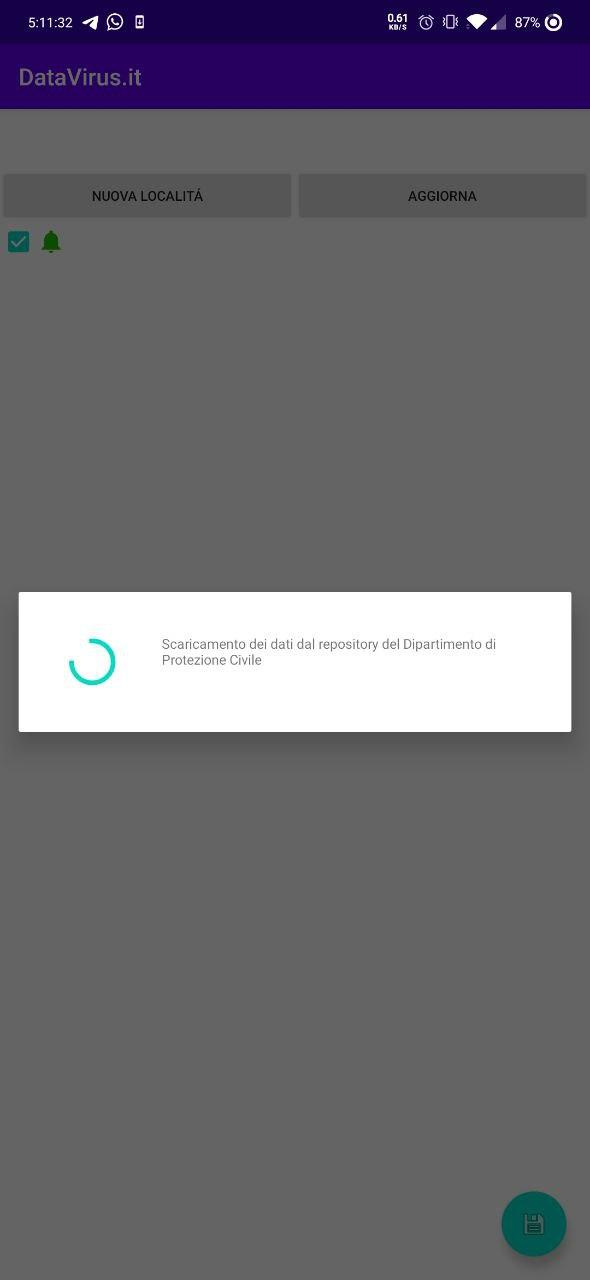
\includegraphics[width=.7\linewidth]{loading_dialog.jpg}
          \caption{Caricamento dei dati}
          \label{fig1:sub1}
        \end{subfigure}%
        \begin{subfigure}{.5\textwidth}
          \centering
          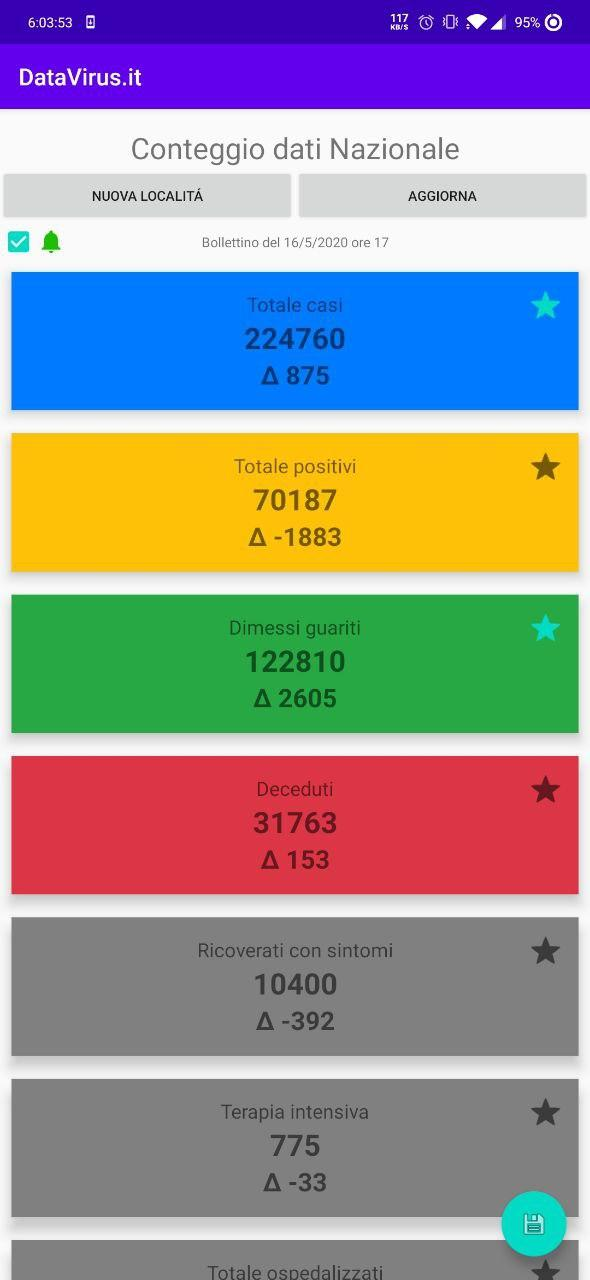
\includegraphics[width=.7\linewidth]{main_activity.jpg}
          \caption{Andamento nazionale}
          \label{fig1:sub2}
        \end{subfigure}
    \end{figure}
    
    Come si puó notare nella figura \ref{fig1:sub2}, questa é la schermata principale dell'applicazione. 
    Viene mostrato in alto la denominazione territoriale dei dati (nella scermata principale verrá mostrato l'andamento nazionale). Sotto i pulsanti, viene visualizzata la data dell'ultimo aggiornamento disponibile dal Dipartimento di Protezione Civile.
    \\
    Il pulsante \quotes{Aggiorna} ricarica i dati dal repository.
    \\
    Vengono poi visualizzate le tile contenenti il dato odierno e la relativa variazione (delta) rispetto alla giornata precedente.
    \\
    \subsection{Implementazione}
    La MainActivity, alla sua creazione, istanzia un oggetto di tipo DataParser.
    La classe DataParser si occupa di eseguire il download dei file JSON dal Dipartimento di Protezione Civile (\textbf{DPC}) in modalitá grafica (verrá visualizzato il dialog che segnala il download in esecuzione. Il dialog utilizzato é \emph{LoadingDialog}).
    \\
    Una volta concluso lo scaricamento, i dati verranno memorizzati in un oggetto di tipo \emph{DPCData}, accedibile dalla callback \emph{onDPCDataReady()} nell'interfaccia \emph{OnDPCDataReady}, o alternativamente dal metodo statico \emph{DataParser.getDPCDataInstance()}.
    \\
    La MainActivity contiene un'istanza di \emph{DataTilesFragment}, che si occupa di visualizzare le tile con i dati (ed incrementi), colorandole e posizionandole in ordine a seconda del parametro 
    (es. la tile \emph{Dimessi guariti} viene sempre colorata di verde e posizionata al terzo posto). Non per tutte le tile é previsto un ordinamento oppure un colore (verrá applicato il grigio come colore di default).
    \\
    Per la lista delle tile scrollabili é stata prevista una RecyclerView (integrata in \emph{DataTilesFragment}). Le tile sono realizzate con un layout CardView.
    Al click su una tile seguirá una chiamata al metodo \emph{onTileClick} presente in una classe che implementa l'interfaccia \emph{OnTileClick}. Nella fattispecie tale classe sará una istanza di \emph{ChartActivity}.

    \section{Cambio zona geografica}
    La denominazione geografica puó essere cambiata premendo sul pulsante \quotes{Nuova localitá} dalla schermata principale (vedi \ref{fig1:sub2}).
    \\

    \begin{figure}[h]
        \centering
        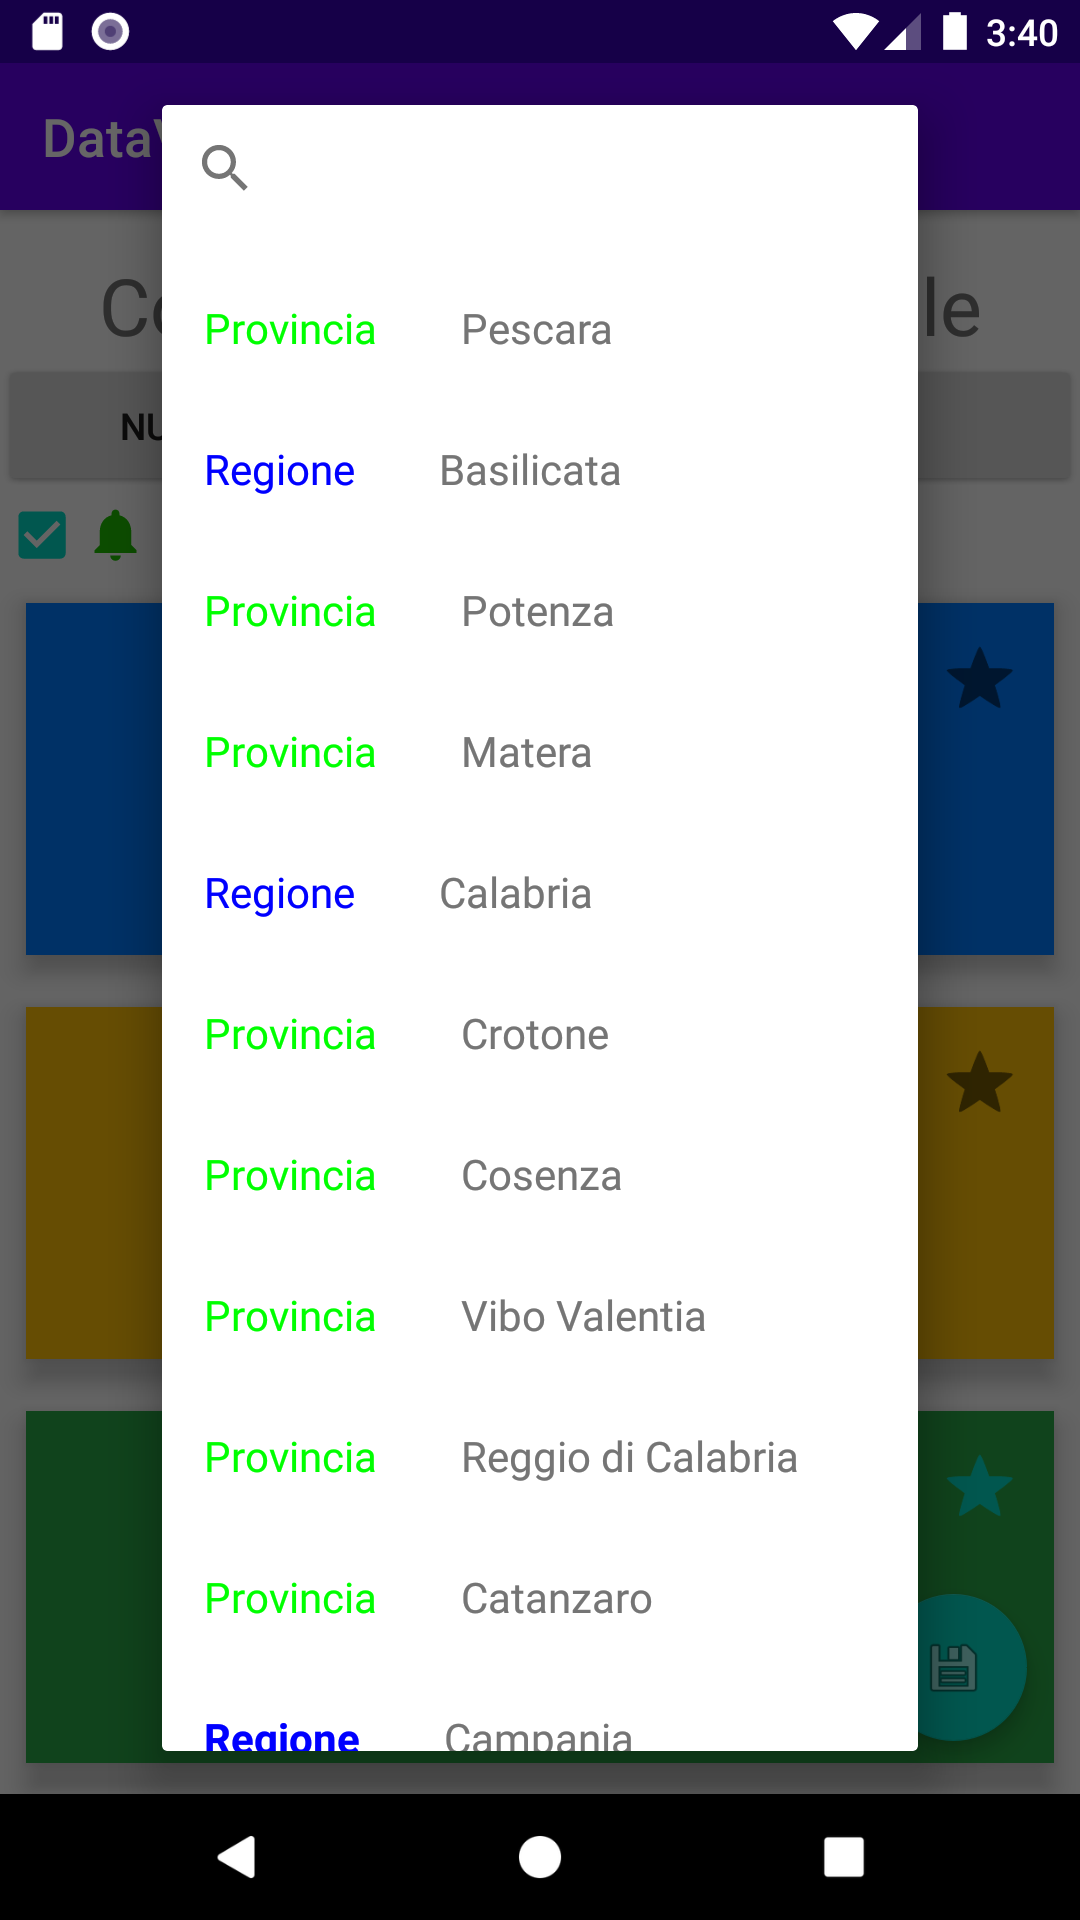
\includegraphics[width=.5\linewidth]{DPC_geo_picker.png}
        \caption{Picker zona geografica}
        \label{fig2}
    \end{figure}

    Grazie al picker si puó scegliere la zona geografica di interesse. Puó essere una provincia, una regione oppure si puó selezionare l'andamento nazionale.
    Per comoditá si puó ulteriormente cercare la zona d'interesse premendo sulla \emph{lente d'ingrandimento}.
    Come risultato verranno visualizzati i dati relativi alla zona selezionata.

    \begin{figure}[h]
        \centering
        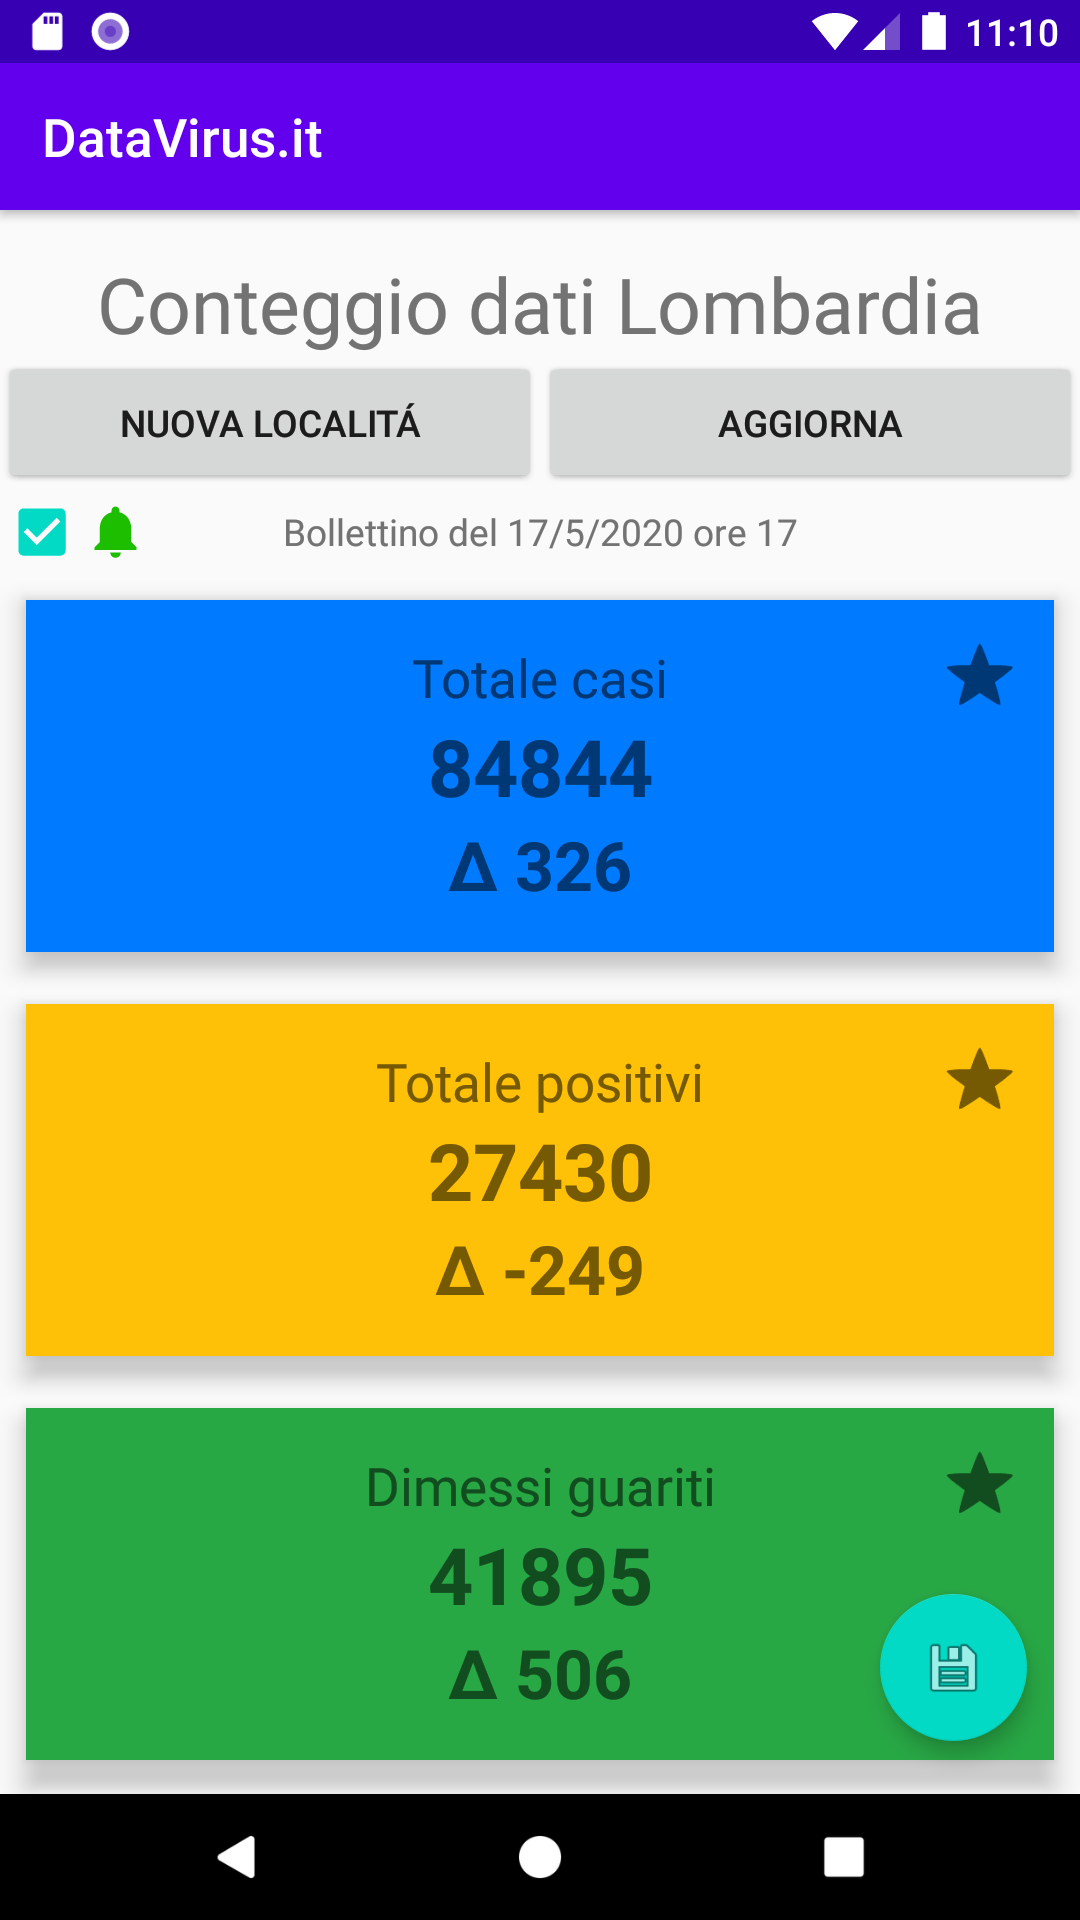
\includegraphics[width=.5\linewidth]{lombardia.png}
        \caption{Esempio visualizzazione regione Lombardia}
        \label{fig3}
    \end{figure}

    Premendo il pulsante back \emph{fisico} si scorreranno all'indietro tutte le selezioni geografiche finora cercate dall'utente.

    \subsection{Implementazione}

    La classe \emph{DPCGeoAdapter} é un'estensione di un DialogFragment che, quando aperto, mostrerá una RecyclerView contenente la lista delle regioni e delle province. In prima posizione si trova la selezione per il dato nazionale.
    \\
    La lista é strutturata in modo che, per ogni regione, ci sia la lista delle province che la compongono nelle posizioni sottostanti. 
    \\
    Alla pressione di una posizione geografica, il GeoPicker chiamerá la funzione \emph{onDPCGeoClick} di una classe che implementa \emph{OnDPCGeoListener} (nella fattispecie verrá utilizzata la MainActivity).
    L'oggetto passato é di tipo \emph{GeographicElement}, il quale descrive il nome dell'ambito geografico e la sua tipologia (\emph{NAZIONALE, REGIONALE, PROVINCIALE}).

    \section{Preferiti}
    Ogni tile ha in alto a destra una \emph{stellina}: quando premuta, la tile relativa viene salvata tra i preferiti.
    Per recuperare la lista delle tile salvate é sufficiente premere sul floating button in basso a destra (visibile nella schermata principale dell'app, \ref{fig1:sub2}).

    \begin{figure}[h]
        \centering
        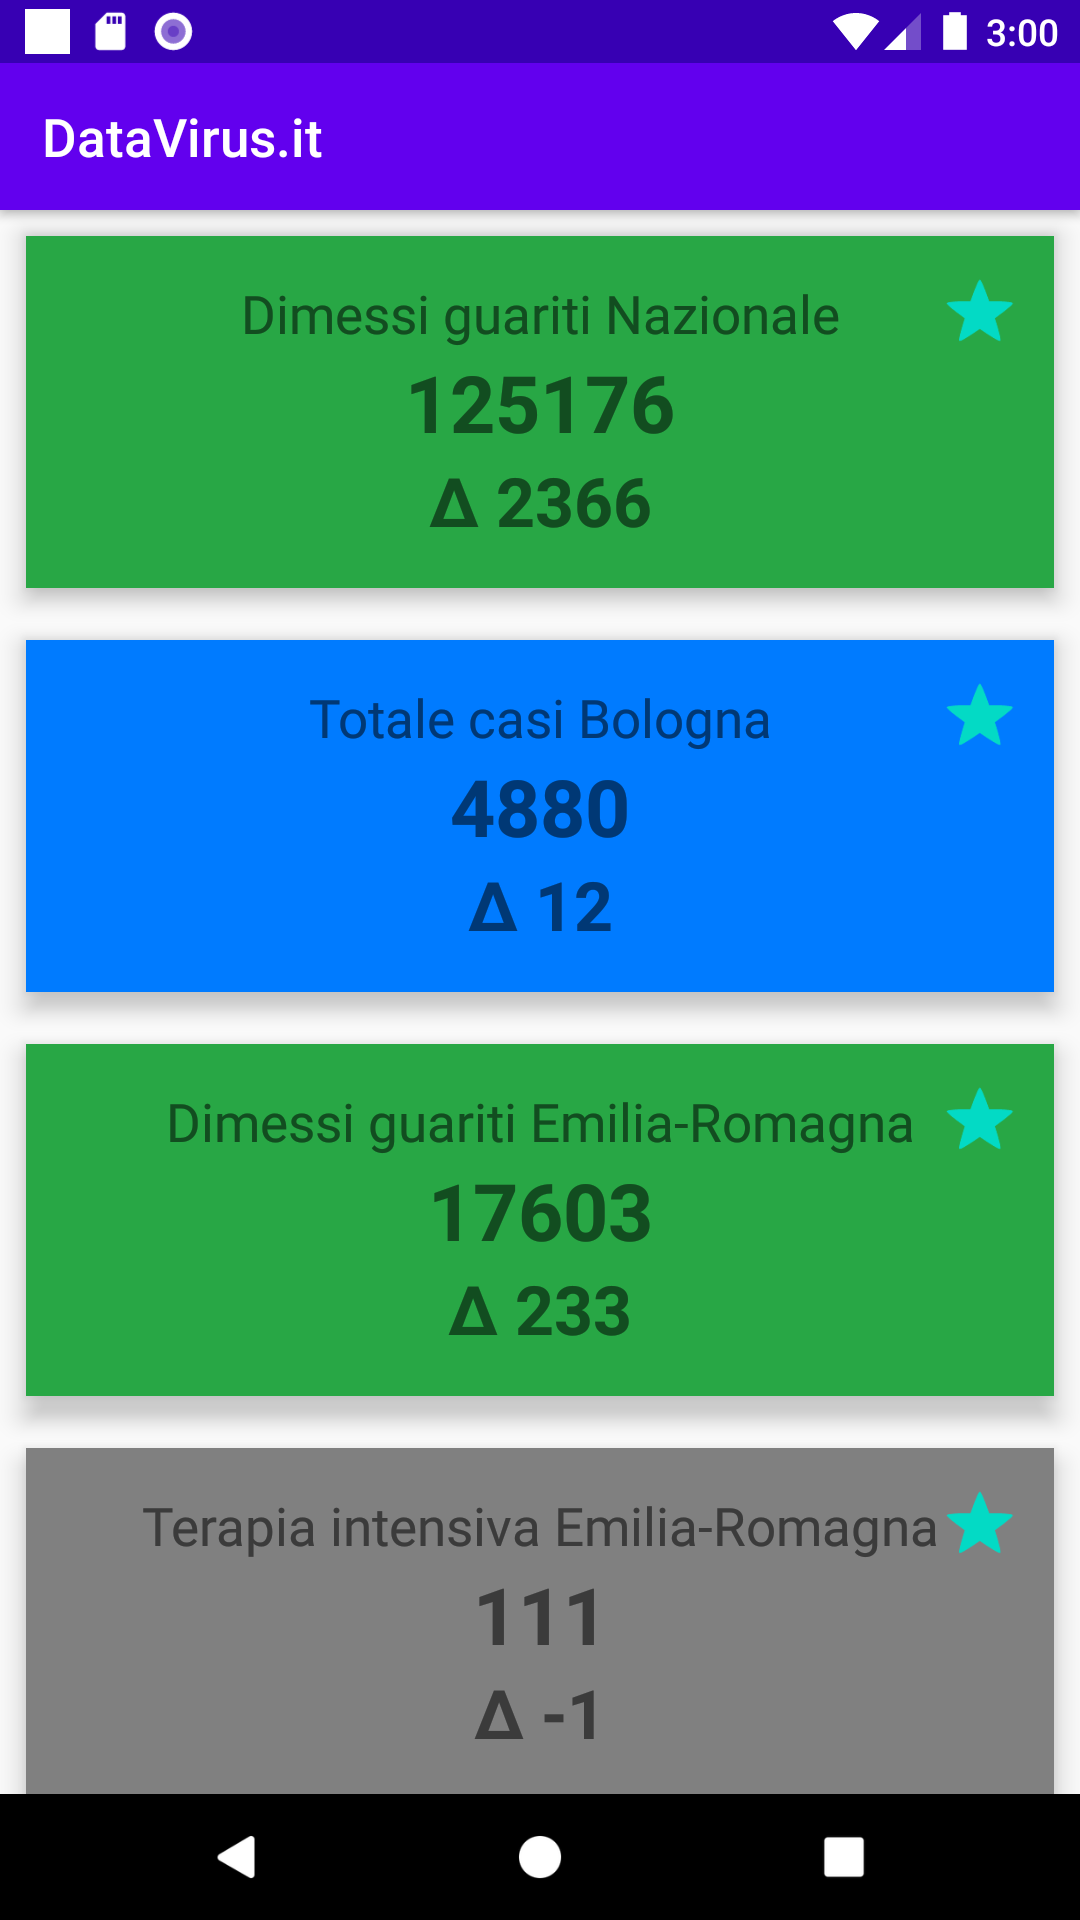
\includegraphics[width=.5\linewidth]{preferences.png}
        \caption{Lista dei preferiti}
        \label{fig4}
    \end{figure}

    Come si puó notare dalla figura \ref{fig4}, le tile salvate sono visualizzate con la loro denominazione geografica a seguito.
    Premendo su una \emph{stellina} precedentemente marcata verrá rimossa tale tile dalla lista dei preferiti.

    \subsection{Implementazione}
    Per il salvataggio dei preferiti si fa uso della classe \emph{ManageStarredTiles}, che offre i metodi per aggiungere o rimuovere un elemento dai preferiti. Per identificare una tile da aggiungere o rimuovere viene passato un oggetto di classe \emph{FieldGeographicElement}.
    \\
    I dati sulle tile marcate come starred vengono salvati in un file privato dell'app, in formato json.
    \\
    Per la visualizzazione della lista delle tile preferite viene utilizzata la \emph{StarredActivity}, che si occupa di istanziare un \emph{DataTilesFragment} che visualizzerá tutte le tile salvate.

    \section{Grafici}
    Ogni qualvolta si premerá su una tile, verrá mostrato l'andamento nel tempo del dato selezionato in un grafico.
    Si presenterá la schermata come quella in figura \ref{fig5:sub1}.
    \\
    Il dato che ora viene mostrato puó essere confrontato con altri dati. Per ottenere questo risultato sará sufficiente premere sul pulsante \quotes{Aggiungi} e selezionare una nuova tile.
    \\
    Ad ogni dato aggiunto viene assegnato un colore random per la sua rappresentazione e apparirá nella lista dei campi attualmente disegnati. 
    Per ciascuno di questi si potrá decidere se nasconderlo o mostrarlo (con la checkbox sulla sinistra) oppure cancellare dalla lista premendo sull'icona del \emph{cestino}.
    \\
    Il grafico é ingrandibile a piacimento, semplicemente utilizzando il \emph{pinch-to-zoom}.

    \begin{figure}[h]
      \centering
      \begin{subfigure}{.5\textwidth}
        \centering
        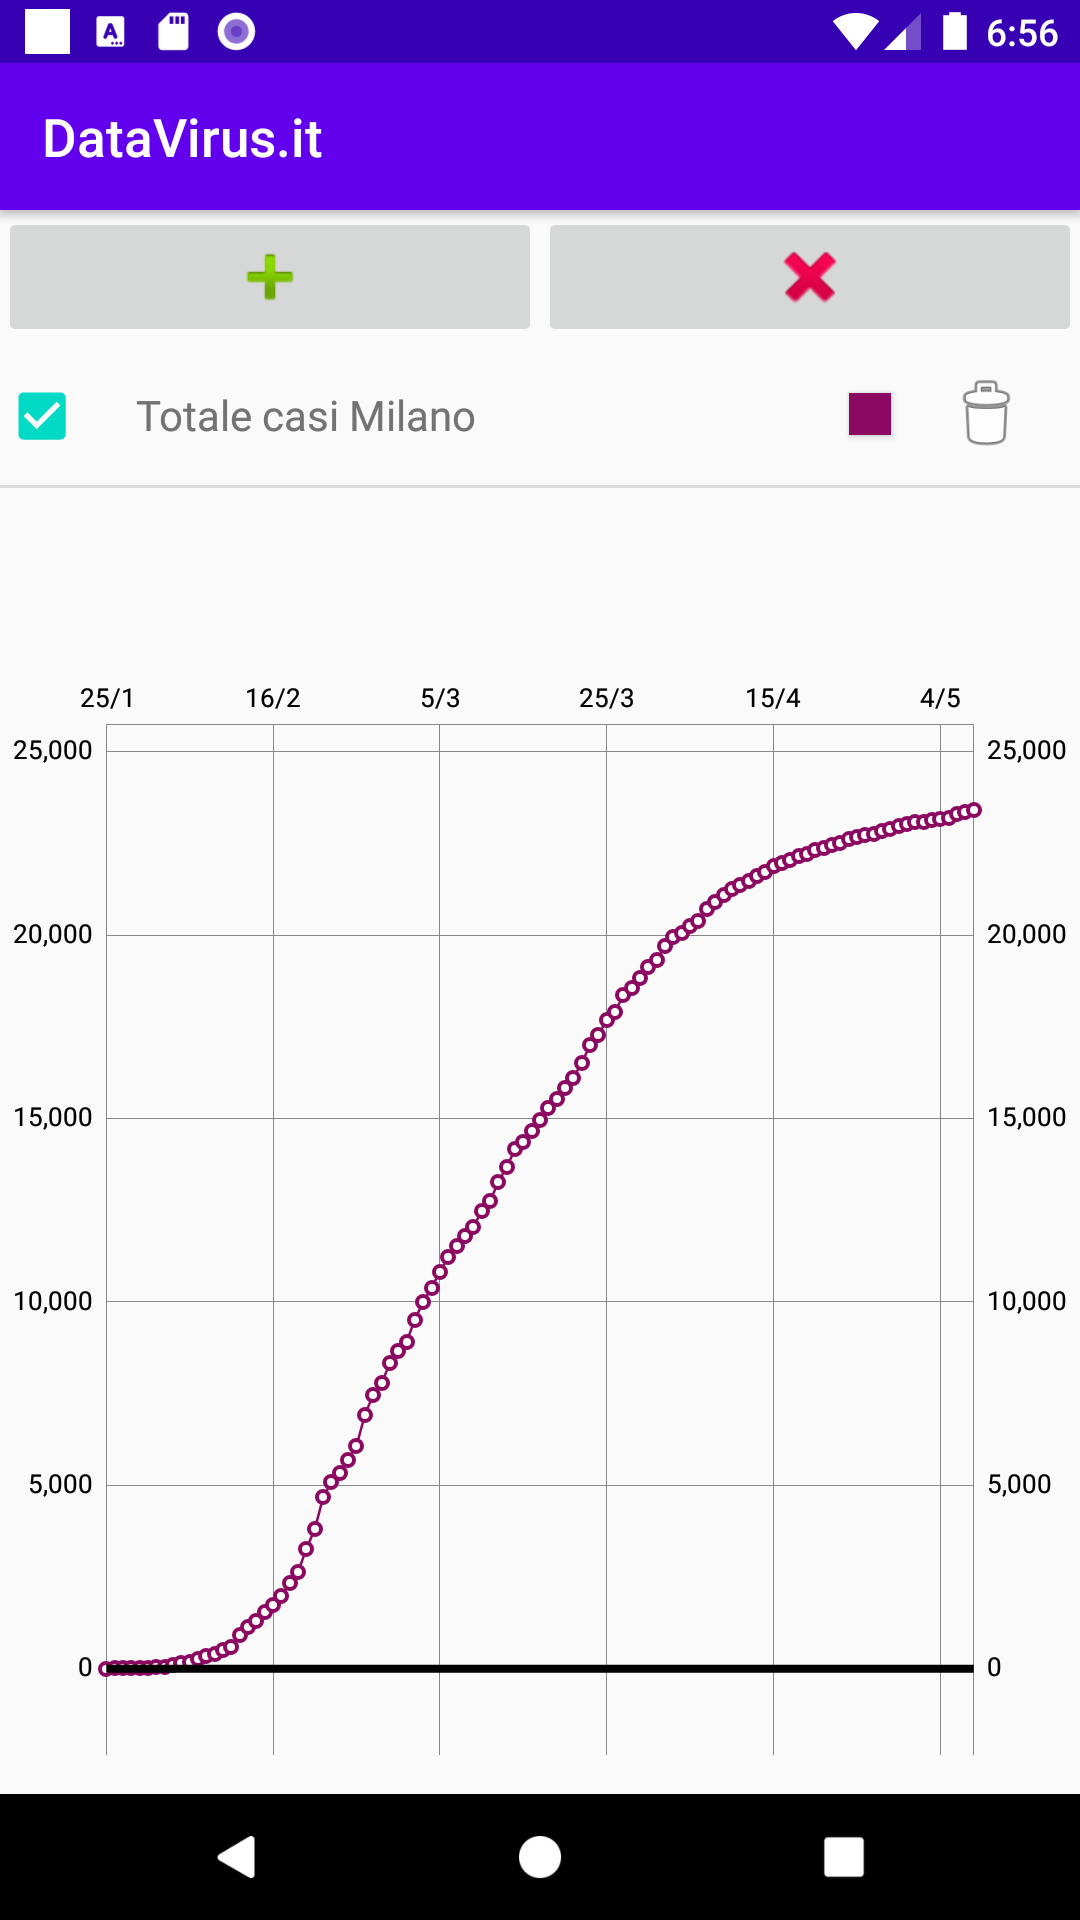
\includegraphics[width=.7\linewidth]{milano.png}
        \caption{Esempio grafico Milano}
        \label{fig5:sub1}
      \end{subfigure}%
      \begin{subfigure}{.5\textwidth}
        \centering
        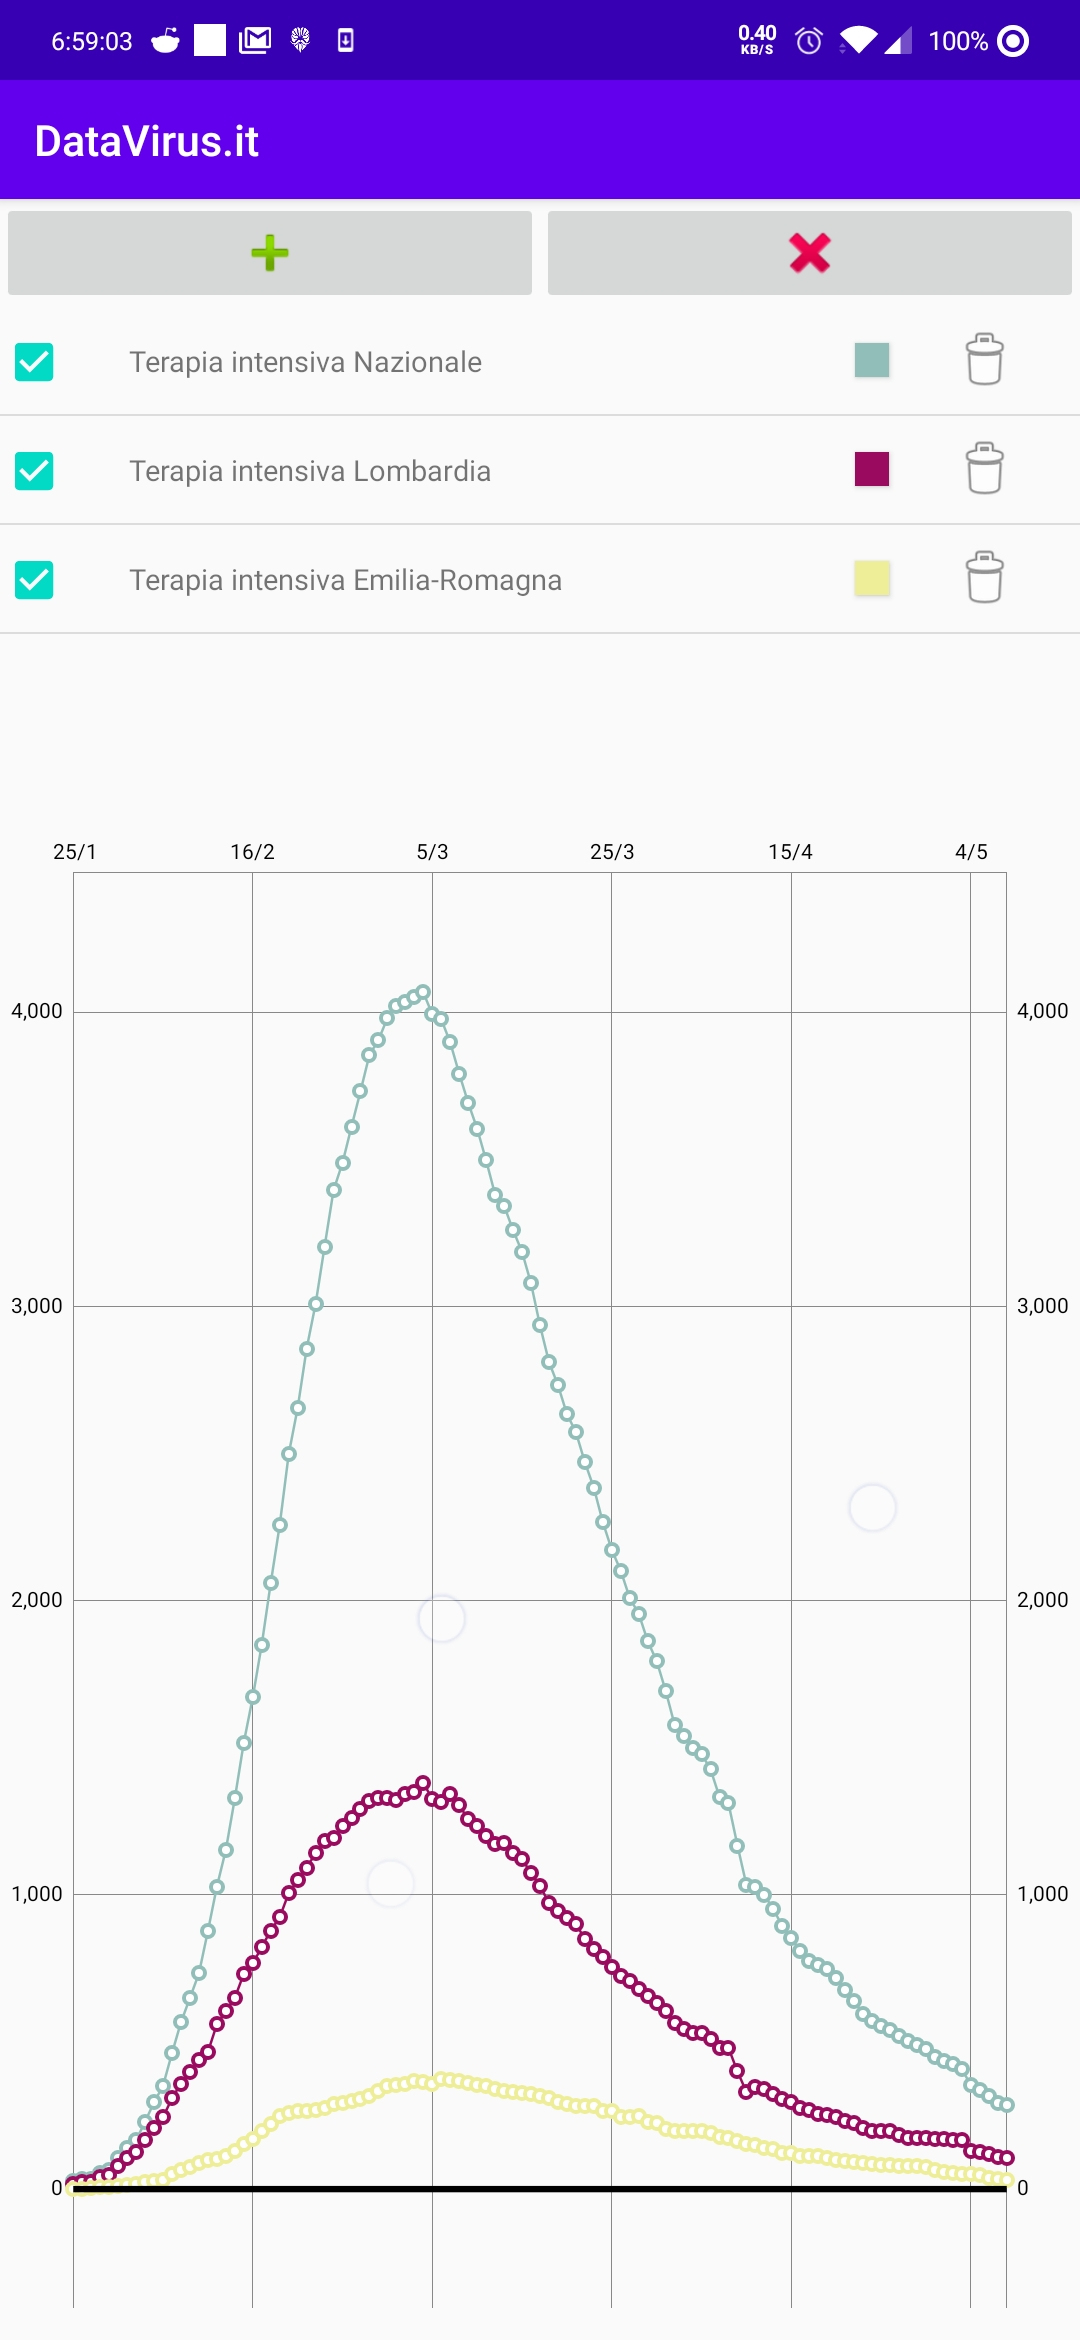
\includegraphics[width=.7\linewidth]{chart_ICU.jpg}
        \caption{Confronto tra terapie intensive}
        \label{fig5:sub2}
      \end{subfigure}
    \end{figure}
    Alla pressione del pulsante \quotes{Pulisci} si chiuderá la schermata del grafico e il grafico attualmente disegnato verrá scartato, insieme a tutti i dati precedentemente immessi.
    Il medesimo risultato si puó raggiungere alla pressione del pulsante back \emph{fisico};

    \subsection{Implementazione}

    Per il grafico é stata utilizzata la libreria \href{https://github.com/PhilJay/MPAndroidChart}{\emph{\textbf{MPAndroidChart}}}, 
    che fornisce un'interfaccia completa per il plotting fornendo molteplici funzionalitá.
    \\
    Questa viene utilizzata dentro alla \emph{ChartActivity}. I dati sono ottenuti attraverso il singleton \emph{ChartModel}, la quale istanza gestisce i dati da disegnare sul grafico.
    L'istanza del singleton \emph{ChartModel} puó essere modificata tramite il fragment \emph{ChartElementsList}, che gestisce la RecyclerView contenente tutti gli elementi aggiunti al grafico e le funzionalitá per nascondere il dato oppure rimuoverlo.
    Il pulsante \quotes{Aggiungi} termina l'activity corrente senza pulire la lista dei dati nel grafico, al contrario del pulsante \quotes{Pulisci} che elimina tutti gli elementi finora aggiunti.
    \\
    Quando si preme su una tile si genera l'\emph{intent} per eseguire \emph{ChartActivity}, passando come extra valori gli elementi contenuti in una istanza di \emph{GeographicFieldElement}.

    \section{Notifiche periodiche}
    Nell'activity principale, a sinistra della data di ultimo aggiornamento, é presente una checkbox con a fianco una campanellina (vedere fig. \ref{fig1:sub2}).
    \\
    Quando marcata, a partire dalle ore 18:00 di ogni giorno, ogni 10 minuti verrá performata una ricerca di nuovi dati aggiornati (orario nel quale il DPC li rende pubblici).
    Nel caso in cui i dati scaricati abbiano data odierna, l'utente verrá avvisato attraverso una notifica. Alla pressione di tale notifica si aprirá l'app.

    \subsection{Implementazione}
    
    Per gestire le notifiche si é fatto uso di una istanza \emph{DataNotifyReceiver}, classe che estende \quotes{Broadcast Receiver}
    che alla sua chiamata istanzia un oggetto di tipo \emph{DataParser} (senza interfaccia GUI) per ottenere dati aggiornati.
    \\
    La chiamata a \emph{DataNotifyReceiver} viene effettuata attraverso un'\emph{intent} performato dall'\emph{AlarmManager}, per impostare l'orario in cui cominciare la ricerca (ore 18:00).
    \\
    Nel caso in cui i dati ottenuti dalla repository GitHub siano aggiornati alla data odierna, \emph{DataNotifyReceiver} invia una notifica all'utente.
    Altrimenti viene impostata l'esecuzione del \emph{DataNotifyReceiver} differita di 10 minuti per una nuova ricerca.

\end{document}